\documentclass{article}

% Pacotes Utilizados -----------------------------------------------------------
\usepackage[utf8]{inputenc}
\usepackage[T1]{fontenc}
\usepackage[brazil]{babel}
\usepackage{sbc-template}
\usepackage{hyperref}
\usepackage{graphicx}

% Dados Pessoais ---------------------------------------------------------------
\title{Análise de \textit{Sites} de Prefeituras Municipais}
\author{Wanderson Camargo\inst{1}\and{}Daniel Perazzoni\inst{1}\and{}Roberto
Raguze\inst{1}}
\address{Centro de Ciências Exatas e Tecnológicas\\
Universidade do Vale do Rio dos Sinos --- UNISINOS
\email{\{wandersonwhcr\and{}dperazzoni\and{}roberto.raguze\}@gmail.com}}

% Corpo ------------------------------------------------------------------------
\begin{document}

\maketitle{}

% Introdução -------------------------------------------------------------------
\section{Introdução}
\label{sec:introducao}

Atualmente, a Internet traz aos seus usuários uma maior velocidade na troca de
informações importantes. Notícias e serviços podem ser acessados rapidamente
através de um \textit{site} ou portal, onde estes dados são exibidos
publicamente ou recebidos através de serviços como \textit{feeders} e
\textit{newsletters}.

O setor público pode utilizar desta facilidade para otimizar alguns serviços
disponíveis de atendimento. Informações como telefone para contato, endereços de
Secretarias ou formulário para solicitação de serviço poderão estar disponíveis
em portal na Internet para o cidadão. Notícias da prefeitura, atuais serviços
prestados ou encontros de representantes com a população tornam o trabalho deste
órgão municipal mais transparente.

Uma \textit{interface} neste caso, deve fornecer uma usabilidade relativamente
acessível para que qualquer pessoa deste município consiga executar tarefas
simples, como consulta de telefones para contato.

Esta proposta de trabalho visa analisar portais de prefeituras municipais da
região metropolitana de Porto Alegre e da região do Vale do Rio dos Sinos. Elas
serão estudadas igualmente, buscando pontos específicos de comunicação com o
cidadão e verificando se o usuário possui uma facilidade ou não de utilização da
sua \textit{interface}.

% Descrição --------------------------------------------------------------------
\section{Descrição}
\label{sec:descricao}

Conforme proposta anterior \cite{camargo2010}, a análise foi feita sobre 3
\textit{sites} de prefeituras municipais da região metropolitana de Porto Alegre
e do Vale do Rio dos Sinos, com foco na qualidade dos serviços prestados ao
usuário final, cidadão residente no município alvo.

\begin{itemize}
  \item Prefeitura Municipal de Porto Alegre
  \item Prefeitura Municipal de Gravataí
  \item Prefeitura Municipal de São Leopoldo
\end{itemize}

\subsection{Assuntos}

Primeiramente, foram tratadas as buscas de informações para contato com os
órgãos da prefeitura, como telefones diretos para serviços ou formulários para
ocorrência de problemas. Num segundo momento, foram discutidas como as notícias
da prefeitura são distribuídas, como são atualizadas e se o conteúdo é
consistente. Após foram analisadas formas de acesso a dados, como leis 
municipais e gastos com recursos públicos atualizados em tempo real, sistema
atualmente chamado \textit{Portal de Transparência}.

% Técnicas Utilizadas ----------------------------------------------------------
\section{Técnicas Utilizadas}
\label{sec:tecnicasutilizadas}

Como estes serviços já estão finalizados e disponíveis, foi aplicada uma
avaliação somativa, levando em consideração a facilidade do uso de seu conteúdo.
O método trabalhado possui características de inspeção de usabilidade, que foi
aplicado em 5 voluntários residentes de cada cidade.

Portanto, como técnica utillizada, temos testes de usabilidades em usuários
finais com preenchimento de questionário previamente formatado. Os três assuntos
foram trabalhados com 6 questões cada, com uma linguagem não técnica, visando
manter o usuário a vontade durante o tempo de respostas.

% Casos Analisados -------------------------------------------------------------
\subsection{Casos Analisados}

\begin{itemize}
  \item Informações
  \begin{itemize}
    \item Disponibilidade do \textit{site} em mecanismos de busca;
    \item Apresentação da página inicial;
    \item Mecanismo interno de busca de conteúdo;
    \item Descrição de todas as seções do \textit{site};
    \item Telefone principal para contato; e
    \item Formulário de contato para sugestões ou dúvidas.
  \end{itemize}
  \item Notícias
  \begin{itemize}
    \item Disponibilidade;
    \item Fácil compreensão;
    \item Atualização periódica;
    \item Notícias por região;
    \item Pesquisa de notícias por conteúdo; e
    \item Impressão das notícias.
  \end{itemize}
  \item Serviços
  \begin{itemize}
    \item Acesso às leis municipais;
    \item Serviços de atendimento ao cidadão;
    \item Acesso ao PROCON;
    \item Acompanhamento de pedido de documentos e protocolo;
    \item Telefones úteis para postos de saúde ou escolas da região; e
    \item Portal de transparência com atualização em tempo real.
  \end{itemize}
\end{itemize}

% Aplicação --------------------------------------------------------------------
\section{Aplicação}
\label{sec:aplicacao}

Foram selecionadas 14 pessoas, distribuídas entre os municípios alvos. Devido a
problemas de comunicação de pessoal, a quantidade de usuários residentes em cada
município ficou disforme.

\begin{itemize}
  \item 9 Usuários da Prefeitura Municipal de Porto Alegre
  \item 4 Usuários da Prefeitura Municipal de Gravataí
  \item 1 Usuário da Prefeitura Municipal de São Leopoldo
\end{itemize}

As pessoas selecionadas responderam um questionário eletrônico
\cite{camargo2010a} com base nos casos analisados na Seção
\ref{sec:tecnicasutilizadas}, aplicados ao \textit{site} do seu município. O
questinário enviado possui 6 perguntas referentes a cada assunto a ser
discutido: informações, notícias e serviços, totalizando 18 perguntas. Cada
pergunta deve receber como resposta um valor entre 1 (difícil utilização) e 3
(fácil utilização).

Conforme as respostas eram enviadas, foram armazenadas em um pequeno banco de
dados para estudo posterior.

% Análise ----------------------------------------------------------------------
\section{Análise dos Dados}
\label{sec:analise}

Para melhor estudo sobre os dados, eles foram analisados primeiramente por
cidade. Cada assunto foi estudado sobre a média aritmética dos valores. O
resultado é discutido posteriormente. A média total da cidade também é gerada e
analisada. Ao final do estudo, a média de todas as cidades é calculada e
verificamos a qualidade dos serviços.

% Prefeitura Municipal de Porto Alegre -----------------------------------------
\subsection{Prefeitura Municipal de Porto Alegre}

\begin{itemize}
  \item \url{http://www.portoalegre.rs.gov.br/}
  \item 9 Usuários
\end{itemize}

\begin{center}
    \begin{tabular}{|c|c|c|c|c|}
        \hline{} Usuário & Informações & Notícias & Serviços & Média Geral\\
        \hline{} 1 & $1,83$ & $2,17$ & $1,83$ & $1,94$\\
        \hline{} 2 & $1,83$ & $2,50$ & $2,00$ & $2,11$\\
        \hline{} 3 & $1,83$ & $2,50$ & $2,00$ & $2,11$\\
        \hline{} 4 & $1,67$ & $2,67$ & $2,00$ & $2,11$\\
        \hline{} 5 & $1,50$ & $1,83$ & $1,83$ & $1,72$\\
        \hline{} 6 & $1,67$ & $1,67$ & $2,00$ & $1,78$\\
        \hline{} 7 & $1,33$ & $1,67$ & $2,00$ & $1,67$\\
        \hline{} 8 & $1,67$ & $1,67$ & $1,83$ & $1,72$\\
        \hline{} 9 & $1,50$ & $2,00$ & $2,50$ & $2,00$\\
        \hline{} Média & $1,65$ & $2,07$ & $2,00$ & $1,91$\\\hline
    \end{tabular}
\end{center}

\subsubsection{Informações}

Podemos verificar que os usuários desta cidade possuem maiores dificuldades em
pesquisa de informações sobre a prefeitura. Se analisarmos os dados brutos,
vemos que o portal não possui um mapa com todas as seções descritas, pois
todos os usuários forneceram a menor nota possível. Os usuários também não
encontraram um formulário para envio de sugestões ou dúvidas. Ainda nas
informações, podemos enfatizar que os usuários encontraram facilmente o telefone
principal da prefeitura.

\subsubsection{Notícias}

O assunto notícias, que possui a melhor nota da pesquisa, recebeu bons valores
quanto ao seu rápido acesso e fácil compreensão. Porém, a pesquisa por bairros e
o sistema de pesquisa das notícias receberam as piores notas.

\subsubsection{Serviços}

Os serviços prestados a população receberam a nota média. Segundo a pesquisa, a
melhor nota vai para o rápido acesso a telefones para contato de setores
públicos. Os usuários forneceram a pior nota para painel de horários de
atendimento, algo importante para comunicação da prefeitura com a sociedade.
Podemos salientar uma grande diferença entre os usuários quanto a pedido de
documentos e acesso a protocolos de solicitação, caracterizando que o serviço
existe, porém muitas pessoas não encontram rapidamente o acesso.

% Prefeitura Municipal de Gravataí ---------------------------------------------
\subsection{Prefeitura Municipal de Gravataí}

\begin{itemize}
  \item \url{http://www.gravatai.rs.gov.br/}
  \item 4 Usuários
\end{itemize}

\begin{center}
    \begin{tabular}{|c|c|c|c|c|}
        \hline{} Usuário & Informações & Notícias & Serviços & Média Geral\\
        \hline{} 1 & $1,67$ & $1,83$ & $1,33$ & $1,61$\\
        \hline{} 2 & $2,00$ & $2,50$ & $1,50$ & $2,00$\\
        \hline{} 3 & $2,00$ & $2,67$ & $2,17$ & $2,28$\\
        \hline{} 4 & $1,83$ & $2,83$ & $1,50$ & $2,06$\\
        \hline{} Média & $1,88$ & $2,46$ & $1,63$ & $1,99$\\\hline
    \end{tabular}
\end{center}

\subsubsection{Informações}

As informações ao cidadão estão com as médias centrais segundo a pesquisa. Ao
analisarmos os dados brutos, podemos verificar que todas as pessoas estão
satisfeitas com a pesquisa do portal em \textit{sites} de busca. Porém, elas não
encontraram um formulário para sugestões e dúvidas. Somente uma pessoa encontrou
o mapa do portal, com descrição de todas as seções e achou de dificuldade média
acessar esta informação.

\subsubsection{Notícias}

As notícias receberam a melhor nota, ganhando destaque na atualização periódica
e versão de impressão com uma boa qualidade. A maior dificuldade das pessoas é
que elas acharam a pesquisa de notícias de seu bairro um pouco difícil e que o
próprio sistema de busca não fornece resultados relevantes.

\subsubsection{Serviços}

Com as piores notas, os serviços prestados à população parecem ser bem precários
e deveriam receber uma maior atenção, principalmente quanto a consulta de
protocolos e pedidos de documentos. Os telefones úteis de setores municipais
também são de difícil acesso, juntamente com o serviço de atendimento ao
consumidor. Algo que podemos relevar é que somente uma pessoa encontrou
facilmente um painel com os horários de atendimento e todas as outras acharam
difícil o acesso.

Um usuário comentou que ``Informações ao Cidadão como PROCON e de direitos estão
difíceis de encontrar e compreender''.

% Prefeitura Municipal de São Leopoldo -----------------------------------------
\subsection{Prefeitura Municipal de São Leopoldo}

\begin{itemize}
  \item \url{http://www.saoleopoldo.rs.gov.br/}
  \item 1 Usuário
\end{itemize}

\begin{center}
    \begin{tabular}{|c|c|c|c|c|}
        \hline{} Usuário & Informações & Notícias & Serviços & Média Geral\\
        \hline{} 1 & $1,33$ & $2,17$ & $2,33$ & $1,94$\\
        \hline{} Média & $1,33$ & $2,17$ & $2,33$ & $1,94$\\\hline
    \end{tabular}
\end{center}

\subsubsection{Informações}

Por imprevistos, somente uma pessoa preencheu o formulário referente a
prefeitura desta cidade. Segundo dados fornecidos, as informações são as que
receberam as menores notas, principalmente quanto à compreensão da página,
qualidade de mecanismos de busca internos, descrição de todas seções do site e
formulário de sugestões e dúvidas.

\subsubsection{Notícias}

As notícias receberam as notas intermediárias, com maior dificuldade em
encontrar notícias sobre um bairro específico. Podemos relevar que os melhores
pontos são que o conteúdo das notícias é de fácil compreensão e elas são
atualizadas periodicamente.

\subsubsection{Serviços}

Os serviços à população estão entre as melhores notas, com ênfase a
disponibilidade de serviços de atendimento ao consumidor e rápido acesso a
telefones úteis. A pior nota vai para o portal de transparência de gastos
públicos.

% Visão Geral ------------------------------------------------------------------
\section{Visão Geral}
\label{sec:visaogeral}

Conforme a Figura \ref{fig:mediapref}, podemos analisar as médias de cada cidade
segundo a satisfação dos usuários entrevistados.

\begin{figure}[ht]
    \centering{}
    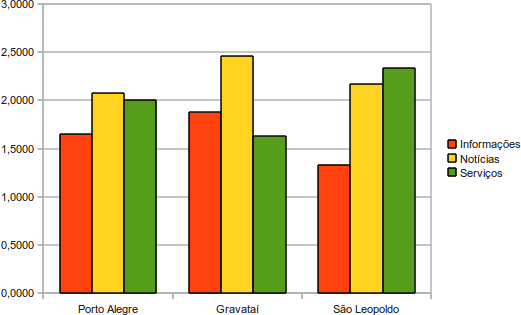
\includegraphics[width=0.8\textwidth]{images/grafico.png}
    \caption{Média de Satisfação dos Usuários dos Portais}
    \label{fig:mediapref}
\end{figure}

A cidade de Porto Alegre possui os valores mais estáveis. Isto é importante pois
todos os setores são alcançados com a mesma intensidade. O maior problema da
cidade são as informações primárias que as pessoas possuem sobre o site,
necessárias para uma primeira necessidade de uso.

O portal da prefeitura de Gravataí possui uma grande diferença entre notícias e
serviços à população. A qualidade das notícias informadas pareceu ser mais
importantes do que serviços à população. Divulgar trabalhos e os serviços nas
ruas está mais forte dentro desta prefeitura do que a execução de serviços
\textit{online}.

Já a prefeitura de São Leopoldo possui uma grande diferença entre informações
primárias e serviços. Isto torna o problema maior, pois se possuirmos serviços
eletrônicos, eles devem sofrer uma divulgação baixa. Porém, devemos lembrar que
estes dados são provenientes de somente uma pessoa e que devem seguir um padrão
maior caso outros usuários sejam entrevistados.

Todas as cidades possuem grandes valores em divulgação de notícias e estes
portais aparentam ser um canal de comunicação de serviços executados pela
prefeitura. Informações básicas recebem uma nota mais baixa e deveriam receber
uma atenção maior para melhorar o conhecimento do \textit{site} por completo.
Serviços eletrônicos, que poderiam evitar filas e automatizar serviços também
deveriam ser melhorados, já que estes portais existem.

\section{Conclusão}

Os \textit{sites} são ferramentas de comunicação ágeis e que podem ser
utilizados para acelerar a distribuição de informações sobre um determinado
assunto. Os portais eletrônicos fornecem a população meios interessantes e
rápidos para conhecer sobre produtos e serviços.

O serviço público pode utilizar desta aplicação para facilitar a vida dos
contribuintes. Uma prefeitura pode além de exibir notícias sobre ações
executadas nos bairros, bem como fornecer serviços, acelerando o atendimento a
população.

Podemos visualizar que as prefeituras desta pesquisa utilizam este método para
otimizar alguns problemas, porém nem sempre todos são alcançados. A preocupação
em exibir notícias da prefeitura e suas ações nas ruas é a mais visível
atualmente, porém outras habilidades podem ser adicionadas a estes portais.

Assim, se todos os pontos aqui estudados fossem aplicados, este órgão público
pode trabalhar com o todo o potencial que um \textit{site} pode trazer, o que
hoje não é feito.

Encontramos muitas dificuldades dos usuários entrevistados, principalmente nos
requisitos de encontrar na \textit{interface} alguns elementos. Verificamos isto
principalmente em questões do formulário totalmente divididas, em pessoas com
muita dificuldade e outras que encontraram facilmente alguma característica.

\subsection{Sugestões}

A prefeitura municipal de Porto Alegre precisa incluir em sua página um acesso
ao mapa do \textit{site}, descrevendo todas as seções disponíveis. Se esta
característica já existe, ela necessita ser melhorada, pois todos os usuários
acharam difícil o acesso. Esta também deve incluir uma tabela com os horários de
atendimento de cada setor à população.

A potencialidade de um portal em acelerar consultas a documentos e solicitações
\textit{online} deve ser revisada na prefeitura municipal de Gravataí,
juntamente com a divulgação de telefones de contato de setores, já que muitos
acharam difícil esta tarefa.

O usuário entrevistado correspondente à prefeitura municipal de São Leopoldo
informou dificuldade quase que completa em todas as questões sobre informações
gerais da prefeitura no portal. O que pareceu mais importante é que a página
inicial não aparenta ser de fácil compreensão, tornando a \textit{interface}
bagunçada.

Todas as prefeituras necessitam incluir um formulário de sugestões e dúvidas
mais visível ao usuário final, pois todas as pessoas entrevistadas informaram
dificuldade.

\subsection{Futuros Projetos}

Um futuro projeto poderia verificar se pessoas com deficiências físicas diversas
possuem um acesso facilitado, características de acessibilidade. O formulário
utilizado também deve ser melhorado, dando a capacidade ao entrevistado de gerar
um pequeno relatório com sugestões.

% Referências ------------------------------------------------------------------
\bibliographystyle{sbc}
\bibliography{sbc-template}

\end{document}